\documentclass[12pt, letterpaper]{article}
\usepackage{graphicx} % Required for inserting images
\usepackage{hyperref}
\usepackage{listings}
\usepackage{amssymb}
\usepackage{amsmath}
\usepackage[english]{babel}
\usepackage{nicefrac, xfrac}
\usepackage{mathtools}
\usepackage[table,xcdraw]{xcolor}
\definecolor{light-gray}{gray}{0.95}
\definecolor{sap}{RGB}{130, 36, 51}
\definecolor{lg}{RGB}{102, 161, 95}
\usepackage[paper=a4paper,left=20mm,right=20mm,bottom=25mm,top=25mm]{geometry}
\newcommand{\code}[1]{\colorbox{light-gray}{\texttt{#1}}}
\newcommand{\codee}[1]{\colorbox{white}{\texttt{#1}}}
\newcommand{\acc}{\\\hphantom{}\\}
\newcommand{\dete}{{\rightarrow}}
\newcommand{\fdot}{{\(\bullet\) }}
\newcommand{\V}{{\mathcal{V} }}
\newcommand{\F}{{\mathcal{F} }}
\newcommand{\Pred}{{\mathcal{P} }}
\newcommand{\comm}[1]{\color{lg}\textit{\hphantom{spaz}// \text{#1}}\color{black}}
\newcommand{\boxedMath}[1]{\begin{tabular}{|c|}\hline \texttt{#1} \\ \hline\end{tabular} :}
\title{Basi di Dati 2}
\author{Marco Casu}
\date{\vspace{-5ex}}
\begin{document}



\maketitle
\begin{figure}[h]
    \centering{
        
\includegraphics[width=1\textwidth ]{images/copertina.jpeg}
    }
\end{figure}
\newpage
\tableofcontents
\newpage
\section{Introduzione}
Questo corso non è ristretto esclusivamente alla progettazione di basi di dati, bensì fornisce
cenni sulla progettazione di software di grandi dimensioni, supportati da basi di dati reali.\acc
Un cliente (committente) fornisce delle specifiche riguardo un progetto che bisogna sviluppare,
esso stesso non sa come verrà implementato o quali sono nello specifico tutte le funzionalità,
un insieme di ingegneri del software, progettisti, e programmatori si occuperanno di "tirare su" il
lavoro completo nel tempo, e varie figure professionali verranno necessariamente coinvolte.\acc
\textit{Tempi per un progetto software complesso} :\begin{itemize}
    \item Capire il problema e cosa vuole realmente il cliente : \(33\%\) del tempo totale.
    \item Progettazione, capire come implementare le richieste del cliente : \(50\%\) del tempo totale.
    \item Effettiva realizzazione (sviluppo del codice) : \(17\%\) del tempo totale.
    \item Del tempo extra per i test di verifica e la manutenzione.
\end{itemize}
\subsection{Contesto Organizzativo}
Le figure professionali \textit{chiave} coinvolte nel progetto sono dette \textbf{attori}, generalmente
sono :\begin{itemize}
    \item Committente ed Esperti del dominio
    \item Analisti e Progettisti
    \item Programmatori
    \item Utenti finali e Manutentori
\end{itemize}
Qual'è la differenza tra analisti e progettisti? E di cosa si occupano gli esperti del dominio?\acc
Il \textbf{dominio} dell'applicazione è l'insieme di informazioni necessarie da conoscere per poter lavorare
ad un progetto che fa riferimento ad uno specifico ambito, ad \textit{esempio}, un applicazione che si occupa
di registrare e gestire le contravvenzioni stradali, vedrà sicuramente nel suo dominio il codice stradale
e le informazioni legislative. \acc L'esperto del dominio è una figura, appunta esperta, del dominio inerente
al progetto in questione, viene pagata dal committente e funge da consulente durante lo sviluppo.
\subsection{Ciclo di Vita del Software}
È possibile suddividere lo sviluppo di un software in macro-fasi principali.\begin{enumerate}
    \item \textbf{Studio di fattibilità} - Ci si approccia al progetto valutando i costi per realizzarlo ed
          i benefici, si pianificano le attività e le risorse del progetto, umane ed economiche, e si individua l'ambiente
          di programmazione hardware e software.
    \item \textbf{Raccolta dei requisiti} - Bisogna capire \textit{cosa il sistema deve fare}, scrivere in prosa
          una documentazione che descriva precisamente le usabilità del progetto, sintetizzando i requisiti, che spesso
          sono contraddittori, trovando i giusti compromessi.
    \item \textbf{Analisi concettuale dei requisiti} - Sono coinvolti gli analisti, che produrranno uno schema
          matematico del progetto, dettagliato per filo e per segno, che definirò cosa l'applicazione deve fare
          indipendentemente dal come. Lo schema prima citato è detto \textit{schema concettuale}, e sarà la base
          da cui partire per la progettazione.
    \item \textbf{Progettazione (design) dell'applicazione} -  Bisogna capire \textit{come} il sistema
          realizzerà le sue funzioni, entra in gioco il progettista, che definirà l'architettura volta ad ospitare
          il software e l'insieme delle tecnologie necessarie.
    \item \textbf{Realizzazione} - Una volta che si hanno le linee guida per la realizzazione, composte
          nelle fasi precedenti, si delega la scrittura del codice ai programmatori, che non sono coinvolti nel resto
          e non devono necessariamente essere a conoscenza di cosa stanno facendo, ma esclusivamente produrre
          le funzioni richieste.
    \item \textbf{Verifica, esercizio e manutenzione} - Le diverse componenti dell'applicazione vengono
          integrate. Una volta che il progetto è realizzato e pronto alla
          messa in esercizio, si passa da una fase di testing ad una fase di utilizzo effettivo, l'applicazione verrà
          monitorata durante l'esercizio ed eventuali correzzione verranno prodotte.
\end{enumerate}
Si osservi il seguente diagramma rappresentante il \textbf{modello a spirale} di realizzazione : \begin{center}
    \includegraphics[width=0.65\textwidth ]{images/cicloDiVita.eps}
\end{center}
Tutto il progetto viene costruito in maniera "iterativa", si dice che lo sviluppo del software sia
\textit{agile}, si comincia raccogliendo i requisiti strettamente necessari, per poi procedere all'analisi
considerando tali requisiti, con l'andare avanti delle fasi portando alla realizzazione di una prima versione
del software, pronta ad essere messa in esercizio, implementante esclusivamente le funzionalità di base, tale
versione renderà chiare le idee al committente che potrà fornire nuovi requisiti, in modo tale da ricominciare il ciclo.\acc
Nulla vieta alle varie fasi di essere eseguite in parallelo, ad esempio, nel tempo \(t_0\) vengono stilati
i requisiti per la prima versione del software, nel tempo \(t_1\) gli analisti iniziano a produrre il modello della versione 1, ma
possono essere nel mentre stilati i requisiti della versione 2, al tempo \(t_3\), com'è di facile intuzione :
Si raccolgono i requisiti per la versione 3, si produce il modello della versione 2, si progetta la versione 1.
\section{Il linguaggio UML}
Il linguaggio UML, acronimo di \textit{Unified Modeling Language}, nasce con l'intento di definire un
linguaggio logico-matematico e formale per la progettazione del software. Utilizza dei diagrammi con lo scopo di
"sintetizzare" un linguaggio puramente logico. \acc
Verrà utilizzato l'UML per modellare il dominio applicativo ed i dati di interesse, utilizzeremo il cosiddetto
\textbf{diagramma delle classi e degli oggetti}. Un \textit{oggetto} modella un elemento del dominio di business,
la cui esistenza è "autonoma", e può essere identificato appunto come un "oggetto" del mondo reale, identifica una classe,
di cui è "estensione", in maniera similare ai linguaggi object-oriented\acc Sarà importante concentrarsi sulle classi
piuttosto che sugli oggetti specifici, una classe definisce un nome identificativo, degli attributi e delle
operazioni.\begin{center}
    \includegraphics[width=\textwidth ]{images/umlBase.eps}
\end{center}
Una classe permette di modellare oggetti dello specifico tipo definito da essa, un oggetto ha un identificatore
univoco (sottolineato), possono però esistere due oggetti identici, a patto che differiscano per
l'identificatore.
\subsection{Associazioni e Link}
Un \textit{associazione} definisce un legame fra due oggetti istanza di due classi diverse, si denota con una freccia o linea che collega due classi,
e deve presentare un titolo, ad esempio, un oggetto di tipo \textit{Libro}, può essere associato ad un oggetto
di tipo \textit{Persona} tramite un'ipotetica associazione \textit{autore}.\begin{center}
    \includegraphics[width=\textwidth ]{images/associazione.eps}
\end{center}
Un \textit{link} non è altro che il corrispettivo delle associazioni, ma sugli oggetti istanza delle classi. Due oggetti
identici possono esistere, ma due link identici fra due oggetti no, si immagini l'esempio precedente di autore,
non avrebbe senso che una persona sia due volte autore dello stesso libro.\begin{center}
    \includegraphics[width=0.8\textwidth ]{images/2link.eps}
\end{center}
\subsubsection{Classi Ponte e Molteplicità}
Si consideri adesso il seguente esempio, si vuole progettare un'applicazione che gestire le prenotazioni di un
hotel, e si produce il seguente modello UML, con le classi \textit{Hotel} e \textit{Persona} unite dall'associazione
"prenota", cosa succederebbe se una persona volesse prenotare 2 volte lo stesso hotel? \begin{center}
    \includegraphics[width=0.7\textwidth ]{images/hotelSbagliato.eps}
\end{center}
Non è giusto modellare la prenotazione come un associazione, in quanto vogliamo che le prenotazioni esistano come
oggetti autonomi, e che uno stesso cliente possa prenotare più volte lo stesso hotel, si necessita di una classe
prenotazione che si occupi di tale relazione, una classe di questo tipo è detta \textbf{classe ponte}, e nel
caso degli hotel, viene
implementata nel seguente modo : \begin{center}
    \includegraphics[width=0.9\textwidth ]{images/hotelGiusto.eps}
\end{center}
Ovviamente, fra le stesse due classi, possono esistere più associazioni diverse, ad esempio, le classi
\textit{Libro} e \textit{Persona}, potrebbero essere relazionate da \textit{autore} ed \textit{editore}. Inoltre,
un oggetto di una classe \(C_1\), può essere collegato tramite link a due oggetti diversi di una stessa classe
\(C_2\), ciò è valido, ma potrebbe causare alcuni errori logici : \begin{center}
    \includegraphics[width=1\textwidth ]{images/multError.eps}
\end{center}
Nonostante lo schema relazionale permetta tali istanze, il fatto che una persona sia nata in due città differenti
non rispetta i vincoli del mondo reale, il diagramma è quindi troppo \textit{lasco}, appositamente per situazioni
di questo tipo, esistono dei costrutti, detti \textbf{vincoli di molteplicità} sulle associazioni, che restringono
il possibile numero delle istanze, imponendo delle restrizioni sul numero di link che possono esistere fra due classi.
\begin{center}
    \includegraphics[width=1\textwidth ]{images/molteplicita.eps}
\end{center}
I vincoli di molteplicità vengono aggiunti ai terminali della linea associazione : \begin{itemize}
    \item il vincolo \textbf{0..*} posto al terminale della classe \textit{A}, in associazione con la
          classe \textit{B} implica che ogni istanza della classe \textit{A}, dovrà essere coinvolta in un numero di link
          dell'associazione in questione, che va da 0 ad un qualsiasi numero (ogni istanza di \textit{A} può essere legata
          ad un numero qualunque di istanze di \textit{B}).
    \item il vincolo \textbf{1..1} posto al terminale della classe \textit{A}, in associazione con la
          classe \textit{B} implica che ogni istanza della classe \textit{A}, dovrà essere coinvolta in un numero di link
          dell'associazione in questione, che va da 1 ad 1 (ogni istanza di \textit{A} sarà collegata ad una sola
          istanza di \textit{B}).
    \item (caso generale) il vincolo \textbf{\(k\)..\(n\)} posto al terminale della classe \textit{A}, in associazione con la
          classe \textit{B} implica che ogni istanza della classe \textit{A}, dovrà essere coinvolta in un numero di link
          dell'associazione in questione, che va da \(k\) ad \(n\).
\end{itemize}\begin{center}
    \includegraphics[width=\textwidth ]{images/esempioAuto.eps}
\end{center}
Si considerino i seguenti requisiti : Si vogliono rappresentare i sovrani
di un regno, di ognuno di loro, è importante considerare il predecessore
ed il successore, è possibile in UML creare un link fra due oggetti della
stessa classe, con un associazione sulla stessa classe : \begin{center}
    \includegraphics[width=0.5\textwidth ]{images/sovrani.eps}
\end{center}
Risulta però \textit{obbligatorio} dare dei nominativi ai \textbf{ruoli}
posti ai terminali dell'associazione, altrimenti sarebbe impossibile quale
delle due classi sta interpretando il ruolo di successore o predecessore.
Vorremmo inoltre che ogni sovrano, eccetto il primo e l'ultimo, abbia esattamente
un successore ed un predecessore, ma il diagramma in questione permette a qualunque
sovrano di violare tali vincoli del mondo reale.
\subsubsection{Associazioni con Attributi}
Si vuole progettare un sistema che gestisca gli esiti (voti in 30esimi) di
più esami sostenuti dagli studenti di un corso di laurea, esisteranno sicuramente
le classi \textit{Studente} ed \textit{Esame}.\acc
Il problema, è che non è possibile utilizzare una classe ponte, in quanto
deve essere impossibile per uno studente, superare lo stesso esame più di una volta. Sarebbe
naturale inserire il voto dell'esame in questa ipotetica classe ponte, ma sapendo che non
è utilizzabile, dove verrà inserito l'attributo \textit{voto}?
\begin{center}
    \includegraphics[width=0.8\textwidth ]{images/votoSbagliato.eps}
\end{center}
Chiaramente, non posso inserirlo nella classe \textit{Studente}, in quanto
ogni studente avrebbe un unico voto per ogni esame, e non posso inserirlo
nella classe \textit{Esame}, dato che tutti gli studenti avrebbero lo
stesso voto nello stesso esame. \acc
È possibile considerare degli \textbf{attributi di associazione}, dando
ad ogni link di \textit{testSuperato}, il corrispettivo valore del voto, risulta
una soluzione naturale, in quanto il voto è assegnato ad ogni superamento di un test :\begin{center}
    \includegraphics[width=0.8\textwidth ]{images/votoGiusto.eps}
\end{center}
Anche se simile, il riquadro \textit{votoSuperato} non rappresenta una
classe, in UML è detta \textit{association class}, e anche essa può essere collegata ad
altre classi, si supponga ad esempio che vogliamo associare ad ogni
test superato, anche il docente che ha verbalizzato il voto, basta
collegare l'associazione con attributi ad una classe \textit{Docente} : \begin{center}
    \includegraphics[width=0.8\textwidth ]{images/conDocente.eps}
\end{center}
\subsection{Tipi di Dato} \label{dataType}
Per ogni attributo di ogni classe abbiamo visto essere necessario
considerare il tipo del dato, esiste infatti un insieme di tipi di
dato \textit{concettuali}, che siano facilmente implementabili
in modo ovvio su qualsiasi sistema o linguaggio di programmazione.\begin{center}
    \code{Intero, Reale, Booleano, Data, Ora, DataOra}
\end{center} Il fatto è che il linguaggio UML vuole modellare situazioni
reali, è quindi necessario considerare dei tipi di dato più restrittivi ed
accurati, nell'esempio precedente degli esami, che tipo di dato dovrebbe
assumere l'attributo \textit{voto}? \acc Non possiamo dargli il tipo "intero",
in quanto ciò permetterebbe ad un voto di assumere anche valori come -5 o 25013, e
non avrebbe alcun senso per essere un voto di un esame. È possibile considerare
dei \textbf{vincoli} con un criterio di \textit{specializzazione}, allo scopo di
restringere l'insieme dei possibili valori che può assumere un determinato
attributo, ad esempio : \begin{center}
    \includegraphics[width=0.7\textwidth ]{images/tipiDato.eps}
\end{center}
In UML, il tipo \(k..n\), indica un \textit{intervallo di numeri interi},
l'attributo in questione può assumere valori da un minimo di \(k\) ad un
massimo di \(n\), nel caso del voto, assume valori da 18 a 30.\acc
È possibile anche definire esplicitamente l'insieme di valori che possono essere
assunti, tramite il tipo \textit{enumerativo} :
\begin{center}
    \includegraphics[width=\textwidth ]{images/enum.eps}
\end{center}
Se volessimo rappresentare un indirizzo? Si possono creare dei tipi di
dato \textbf{composti}, costituiti da più tipi di dato, con le eventuali
restrizioni (è possibile definire i tipi di dato in un documento separato) :
\begin{center}
    \includegraphics[width=\textwidth ]{images/datiComposti.eps}
\end{center}
Possono essere definiti anche dei \textit{vincoli di molteplicità} sugli
attributi, permettendo ad un oggetto di avere più campi di uno stesso attributo, ad
esempio, una classe \textit{Utente} di un social network, può permettere ad ogni utente di
avere più indirizzi email, allora l'attributo si definirà nel seguente modo : \begin{center}
    email : String [1..*]\comm{uno o più indirizzi email}
\end{center}
\subsection{Vincoli}
Il linguaggio UML permette di aggiungere i cosiddetti \textbf{vincoli d'integrità}, delle asserzioni che hanno lo
scopo di restringere il possibile insieme delle istanze, ossia degli oggetti ammessi. Una tipologia di vincolo è
quella dell'\textit{identificazione di classe}, è un vincolo che, impone a due differenti istanze di una classe,
di non poter avere uno o più attributi coincidenti.\acc
Un tipico esempio può essere fatto per una classe \code{Persona}, che presenta un attributo \code{codice fiscale},
è necessario un vincolo di identificazione di classe, che imponga a due differenti istanze di \code{Persona} di non
avere lo stesso \code{codice fiscale}. \acc Tale vincolo può essere aggiunto anche su un insieme di attributi,
se il vincolo è su \code{x} ed \code{y}, due oggetti istanza possono coincidere su \code{x} ma non su \code{y}, oppure
su \code{y} ma non su \code{x}, non possono essere coincidenti su entrambi.\begin{center}
    \includegraphics[width=\textwidth ]{images/identificazione.eps}
\end{center}
Affianco all'attributo in questione, si inserisce la dicitura \code{\{id\}}, possono coesistere anche identificazioni
di classe differenti, di solito si usano le diciture \code{\{id1\}, \{id2\}...,\{id$k$\}} ecc.\acc Un vincolo di
identificazione può anche coinvolgere un'associazione. Se il vincolo è posto su un'associazione da
\code{x} ad \code{y}, e su un attributo
della classe \code{x},
vuol dire che non possono esistere due istanze di \code{x} con l'attributo in questione coincidente, che hanno un
link verso la medesima istanza di \code{y} :\begin{center}
    \includegraphics[width=\textwidth ]{images/vincoloAss.eps}
\end{center}
Attenzione : Un vincolo di identificazione di classe può coinvolgere esclusivamente attributi a molteplicità
$1..1$ e associazioni in cui il ruolo della classe ha molteplicità $1..1$.
\subsection{Generalizzazione delle Classi}
Risultano molto comuni, situazioni in cui diverse classi condividono gli stessi attributi. Il concetto di classe e sotto-classe
è ben noto, già dal corso di
\color{blue}\href{https://github.com/CasuFrost/University_notes/blob/main/Primo%20Anno/Secondo%20Semestre/Metodologie%20di%20Programmazione/Appunti%20Metodologie%20di%20programmazione.pdf}{
    Metodologie di Programmazione
}\color{black}, dove si è affrontata la programmazione orientata agli oggetti, in UML, è possibile definire delle relazioni
di classe e sotto-classe, che però risultano ben più "potenti" e flessibili del corrispettivo in Java.\begin{center}
    \includegraphics[width=\textwidth ]{images/sottoclasse..eps}
\end{center}
Tutti gli attributi, associazioni e le molteplicità della superclasse sono ereditati dalla sottoclasse. Ovviamente
la relazione di classe-sottoclasse può essere re-iterata, costruende un "albero" gerarchico, in cui ogni
livello eredita gli attributi ed associazioni del livello superiore.\acc La classe \code{Studente} sarà sottoclasse di
una classe \code{Persona}, se quest'ultima è in una associazione \code{nascita} con una classe \code{Città}, anche
\code{Studente} lo sarà, una sottoclasse di \code{Studente}, ad esempio, \code{StudenteStraniero}, erediterà sia
le proprietà di \code{Studente} che quelle di \code{Persona}. \begin{center}
    \includegraphics[width=0.6\textwidth ]{images/studStraniero.eps}
\end{center}
Tutto ciò, aumenta significativamente la complessità dello schema relazionale e del livello degli oggetti, nulla vieta
ad un oggetto di appartenere a più classi, nell'esempio precedente, un istanza di \code{StudenteStraniero}, è anche
istanza di \code{Studente} e \code{Persona}, però la classe più \textit{specifica} alla quale fa riferimento è appunto
\code{StudenteStraniero}, si definisce per un oggetto quindi l'insieme delle sue classi più specifiche.
\begin{center}
    \includegraphics[width=0.8\textwidth ]{images/ClassiSpec.eps}
\end{center}
Se diverse classi sono sottoclassi di una classe comune, è possibile utilizzare il costrutto "\textit{is-a}" per
denotare tale comportamento del modello. Si ha una classe \code{a}, e due classi \code{b} e \code{c}, entrambe
sottoclassi di \code{a} tramite il costrutto "\textit{is-a}", un oggetto istanza di \code{a} potrà essere anche :\begin{itemize}
    \item Sia istanza di \code{b} che di \code{c}.
    \item Solo istanza di \code{b}.
    \item Solo istanza di \code{c}.
    \item Ne istanza di \code{b}, ne di \code{c}.
\end{itemize}\begin{center}
    \includegraphics[width=0.7\textwidth ]{images/isa.eps}
\end{center}
In questo caso \code{Studente} e \code{Lavoratore} fanno parte della \textbf{stessa generalizzazione}, ossia \code{occupazione},
nulla vieta ad una classe di essere superclasse di generalizzazioni distinte : \begin{center}
    \includegraphics[width=0.7\textwidth ]{images/isa2.eps}
\end{center}
In questo modello, una Persona può essere : Uomo, Donna, Uomo e Donna, ne Uomo ne Donna, e contemporaneamente
può essere Studente, Lavoratore, Studente e Lavoratore o nessuno dei due. Risulta ambiguo il fatto che una persona
possa essere sia uomo che donna, è necessario imporre allo schema, che ogni persona sia o Uomo o Donna, è possibile
considerare dei \textbf{criteri sulle generalizzazioni}, che si occupano proprio di gestire queste situazioni.\begin{itemize}
    \item \textbf{Criterio disjoint} - Impone agli oggetti istanza di una classe soggetta a generalizzazione, di non poter
          essere istanza di più di una delle sottoclassi in questione. Se nell'esempio precedente, la generalizzazione
          \code{genere} avesse il criterio \textit{disjoint}, sarebbe impossibile essere sia Uomo che Donna, ma
          sarebbe ancora possibile non essere ne Uomo ne Donna.
    \item \textbf{Criterio complete} - Impone agli oggetti istanza di una classe soggetta a generalizzazione,
          di dover essere obbligatoriamente istanza di almeno una delle sottoclassi in questione. Se nell'esempio precedente, la generalizzazione
          \code{genere} avesse il criterio \textit{complete}, sarebbe impossibile non essere ne Uomo ne Donna, ma
          sarebbe ancora possibile non essere sia Uomo che Donna.
\end{itemize}
A seguito di ciò, è possibile combinare i diversi criteri per poter permettere ad un istanza di persona, di essere
necessariamente o Uomo o Donna. Vogliamo quindi che la generalizzazione \code{genere} consideri entrambi i criteri
complete e disjoint, vogliamo invece che la generalizzazione ruolo non abbia criteri, in quanto è possibile che una
persona decida di studiare, lavorare, fare entrambi o non fare nulla. \begin{center}
    \includegraphics[width=1\textwidth ]{images/isa3.eps}
\end{center}
Ora le possibili combinazioni di persona sono 8 : Studente Uomo,
Lavoratore Uomo,
Studente e Lavoratore Uomo,
Nullafacente Uomo,
Studente Donna ,
Lavoratore Donna,
Studente e Lavoratore Donna e
Nullafacente Donna.\begin{center}
    \includegraphics[width=1\textwidth ]{images/criteriDisjointComplete.eps}
\end{center}
UML permette anche ad una classe di ereditare da più classi, anche se tale scelta potrebbe
aumentare troppo la complessità del diagramma, e va utilizzata esclusivamente quando necessario, molto spesso
è consigliabile procedere diversamente.\begin{center}
    \includegraphics[width=0.85\textwidth ]{images/eredMultipla.eps}
\end{center}
\subsection{Operazioni di Classe}
Una classe ha un nome, degli attributi e delle \textit{operazioni},
esse definiscono il comportamento della classe e differentemente dagli attributi
non sono statici.\begin{center}
    \includegraphics[width=0.75\textwidth ]{images/operazione.eps}
\end{center}
Un operazione è una proprietà il cui valore è calcolato a
partire dai valori dell'oggetto che la invoca od altri oggetti ad esso
correlati, un operazione puà anche cambiare lo \textit{stato} di un
oggetto. Quando un operazione modifica un oggetto, si dice che provoca degli
\textit{effetti collaterali}.\acc
La sintassi è la seguente, un operazione ha un \textit{nome}, dopo di ché
si specificano in delle parentesi tonde i parametri con relativi tipi, alla fine
si inserisce il tipo di ritorno dell'operazione. L'operazione definita in
una classe $x$ viene sempre invocata da un oggetto istanza di $x$. L'ereditarietà
ovviamente, si applica anche alle operazioni.\acc
in UML quindi vengono definite le operazioni con i loro nomi (evocativi), parametri e tipo di ritorno, ma non viene
esplicitato in maniera formale cosa queste operazioni devono calcolare. La descrizione logica-formale di ciò che
le operazioni devono fare (non come), viene data in un documento separato.
\subsection{Documenti di Specifica}
Tali \textit{specifiche} hanno lo scopo di affiancare il diagramma UML, e sono contenute in un documento separato, un tipo
di specifiche già presentate sono le specifiche dei \textbf{tipi di dato}, viste nel capitolo \ref{dataType}, esistono
4 documenti differenti per le specifiche.
\subsubsection{Specifica delle Classi}
La specifica delle classi è un documento che associa ad ogni classe, appunto, una specifica formale su ciò che rappresenta, di cui
per ogni operazione è data la sua descrizione logica-matematica, tale specifica può essere scritta in linguaggio
umano (informale) ed in linguaggio puramente logico (formale), per ora vedremo degli esempi di specifiche
informali.\acc
La specifica di un operazione segue il seguente template : \begin{quote}
    nome\_operazione(parametri) : tipo\_ritorno\begin{itemize}
        \item pre condizioni  \\\(\dots\)\\\(\dots\)\\\(\dots\)
        \item post condizioni  \\\(\dots\)\\\(\dots\)\\\(\dots\)
    \end{itemize}
\end{quote}
Le specifiche includono alcune parole chiave, come \code{this}: L'oggetto invocante, oppure
\code{result}: Il valore di ritorno.\acc
Le \textbf{post condizioni} danno la definizione matematica dell'operazione e del valore che restituiranno,
omettendo eventuali meccanismi di calcolo o implementazioni. Deve essere segnalato se l'operazione
modifica o no il livello degli oggetti (le istanze presenti).\acc Le \textbf{pre condizioni} sono le condizioni
che devono essere soddisfatte dalle istanze per far si che l'operazione possa essere
invocata, definiscono il cosiddetto \textit{contratto} dell'operazione, va anche specificato se l'operazione
modifica o no il livello degli oggetti.\begin{center}
    \includegraphics[width=0.8\textwidth ]{images/specificaClassi.eps}
\end{center}
\subsection{Specializzazione}
Abbiamo visto come una classe può essere generalizzata, in un rapporto padre-figlio, ossia superclasse-sottoclasse, e
che la classe figlia eredita gli attributi e le operazioni della classe padre, il punto è che, essa può anche
\textit{specializzare} un attributo desiderato, ossia \textit{restringerne} il dominio, ad esempio:
\begin{center}
    \includegraphics[width=0.75\textwidth ]{images/specAttributo.eps}
\end{center}
Nel modello sovrastante, un articolo in vendita potrebbe avere una garanzia valida per zero o più anni, ma un articolo nuovo
ha una garanzia di minimo due anni, il tipo specializzato deve essere un \textbf{sottotipo}, vale a dire che l'insieme
dei possibili valori che l'attributo specializzato può assumere, deve essere un sotto-insieme dell'insieme dei valori che può
assumere l'attributo che specializza, si dice che ne \textit{restringe} il tipo.\acc
Anche un association class, essendo una classe, può essere specializzata ed essere soggetta a generalizzazioni.
\begin{center}
    \includegraphics[width=0.75\textwidth ]{images/specAssociazione.eps}
\end{center}
In questo modello, ogni articolo è venduto da esattamente un utente, e gli articoli nuovi possono essere venduti
esclusivamente da venditori professionali. Un articolo nuovo è in associazione con un utente, tale associazione però
può essere sia \textit{venditore} che \textit{venditoreNuovo}, nel secondo caso, l'utente deve essere necessariamente
un venditore professionale.\acc
Supponiamo che vi sia una specializzazione di articolo, ossia un articolo in offerta, il calcolo del suo prezzo deve
essere soggetto ad una riduzione, ha senso che vi siano due differenti operazioni \textit{calcoloPrezzo} e
\textit{calcoloPrezzoOfferta}? No, dal momento che è possibile \textit{specializzare un operazione}, distinguendo
le specifiche, eventualmente anche rendendo completamente differenti le post-condizioni. \begin{center}
    \includegraphics[width=\textwidth ]{images/specOperazione.eps}
\end{center}
L'importante è che l'operazione specializzata, rispetto a quella che specializza, mantenga:\begin{itemize}
    \item Lo stesso numero e tipo di argomenti.
    \item Lo stesso tipo di ritorno, oppure un sotto-tipo del tipo dell'operazione che spacializza.
\end{itemize}
\subsection{Specifica dei Vincoli Esterni}
Ci sono delle regole che il solo diagramma UML non può modellare, si definiscono
quindi delle costrizioni \textit{esterne} al diagramma, in un documento separato,
che hanno lo scopo di \textbf{restringere} il possibile livello degli oggetti,
con dei requisiti più \textbf{sofisticati}.\begin{center}
    \includegraphics[width=0.75\textwidth ]{images/vincoliEsterni.eps}
\end{center}
In tale modello, voglio far si che i direttori di un dipartimento, ne afferiscano,
da almeno 5 anni, il diagramma UML non permette di modellizzare tale vincolo.\acc
Un vincolo esterno è composto da:\begin{itemize}
    \item Un identificatore univoco per riferirsi al vincolo.
    \item Un'asserzione matematica/logica, un invariante sui dati, ossia delle
          condizioni che i dati devono necessariamente rispettare.
\end{itemize}
Per semplicità, inizialmente le asserzioni saranno scritte in linguaggio
umano. Se un vincolo coinvolge una sola classe, per mantenere un certo grado di
modularità, è buona norma specificare tale vincolo all'interno del documento
di specifica della classe in questione.
\subsection{Diagramma degli Use-Case}
Insieme all'UML, si modella un diagramma che descrive le funzionalità che il sistema deve realizzare, in termini appunti 
di use-case (scenari di utilizzo), tali use-case possono essere desritti come l'insieme omogeneo di 
\textit{funzionalità} che un \textit{determinato gruppo} di utenti omogeneo può compiere. Tipicamente coinvolge 
concetti rappresentati da più classi ed associazioni del diagramma delle classi.\acc 
Definiamo come \textbf{attore}, il ruolo o la categoria che un utente del sistema (oppure un sistema esterno) può assumere interagendo 
con il sistema. Un singolo utente può assumere più ruoli, ossia può essere rappresentato da più attori, e diversi utenti 
possono essere rappresentati dallo stesso ruolo, ossia essere rappresentati dallo stesso attore.\begin{quote}
    \textit{Esempio} : Un sistema prevede due attori : Docenti e Studenti. Paolo può essere sia Docente che Studente, mentre 
    sia Alice che Giovanni sono entrambi Studenti.
\end{quote}
\subsubsection{Semantica del Diagramma}
UML fornisce il diagramma degli use-case, è un \textit{grafo}, in cui:\begin{itemize}
    \item I \textbf{nodi} rappresentano attori e use-case. 
    \item Gli \textbf{archi} rappresentano:\begin{itemize}
        \item $(i)$ - La possibilità per un attore di invocare uno use-case (a quali funzionalità può accedere un attore).
        \item $(ii)$ - La possibilità per uno use-case di invocare un altro use-case.
        \item $(iii)$ - La generalizzazione fra attori e fra use-case (verrà vista in seguito).
    \end{itemize}
\end{itemize}
Gli attori sono rappresentati con uno \textit{stickman}, gli use case da un ellisse.\begin{center}
    \includegraphics[width=0.9\textwidth ]{images/use-case.eps}
\end{center}
\textbf{Attenzione} : Il fatto che esista un attore \textit{Utente} non implica necessariamente l'esistenza di un 
una classe \underline{Utente} nel diagramma delle classi, avremmo la già citata classe \underline{Utente} 
\textit{esclusivamente} se  il sistema deve rappresentare dei \textit{dati} (attributi) sugli utenti.\acc 
Vediamo adesso un \textit{Esempio} di un diagramma degli use-case. Si hanno le seguenti specifiche: \begin{quote}
Il sistema deve permettere agli studenti di iscriversi, via web, ai corsi offerti. La segreteria deve poter
assegnare i docenti ai singoli corsi. I docenti devono poter inserire i risultati dei test degli studenti: tali
test sono somministrati agli studenti utilizzando il sistema.\end{quote}\begin{center}
    \includegraphics[width=0.9\textwidth ]{images/esempioUse-case.eps}
\end{center}
Note sugli use-case:\begin{itemize}
    \item \textit{Gestione iscrizioni} : funzionalità che permettono l'iscrizione via web da parte degli studenti.
    \item \textit{Gestione test} : funzionalità che permettono la creazione, la somministrazione e la valutazione 
    dei test.
    \item \textit{Gestione docenti} : funzionalità che permettono l'assegnazione dei docenti ai corsi.
\end{itemize}
Ogni singolo utente che si interfaccia/interagisce con il sistema modellato deve necessariamente assumere uno  
fra questi ruoli. Anche se esiste l'attore \textit{Segreteria}, nel diagramma delle classi potrebbe non esistere alcuna 
classe \underline{Segreteria}, in quanto di essa non è necessario salvare alcuna informazione.\acc 
Nel diagramma sovrastante sorge un problema, sia l'attore \textit{Studente} che \textit{Docente} hanno accesso 
a tutte le funzionalità dello use-case \textit{Gestione test}, e non solamente a quelle che li riguardano. Nel diagramma, 
il concetto di \textbf{Inclusione}, permette ad uno use-case di utilizzare \textit{alcune} delle funzionalità 
di un altro use-case.\begin{center}
    \includegraphics[width=\textwidth ]{images/inclusione.eps}
\end{center}
In questo modello, l'attore \textit{Docente} come l'attore \textit{Studente} ha un accesso limitato alle funzionalità dello 
use-case \textit{Gestione test}, i docenti potranno creare e valutare i test, e gli studenti potranno parteciparvi, 
\textit{Gestione test} include le funzionalità che permettono la memorizzazione nel sistema dei test e delle 
risposte degli studenti.\acc 
Ci sono delle situazioni in cui uno use-case, eredità le funzionalità di un'altro use-case, aggiungendone di nuove,
tale concetto prende il nome di \textbf{Estensione}. Riguardo il modello precedente, supponiamo che uno studente che 
si iscrive ad un test, ha anche la possibilità, se volente, di pagare online, 
lo use-case \textit{Iscrizione} verrà quindi esteso. Il pagamento online è un caso particolare di iscrizione.
\begin{center}
    \includegraphics[width=0.8\textwidth ]{images/estensioneUse-case.eps}
\end{center}
Alcuno funzionalità di uno use-case, in alcuni casi particolari, possono essere \textit{rimpiazzate} con le 
funzionalità di un'altro use-case, è possibilie \textbf{generalizzare uno use-case}. Supponiamo che gli studenti devono 
potersi identificare, e tale identificazione può avvenire tramite una password, oppure tramite un accesso biometrico 
(impronta digitale o iride):\begin{center}
    \includegraphics[width=0.8\textwidth ]{images/useCasegeneralizzazione.eps}
\end{center}
\textit{Nota} : nei diagrammi degli use-case non possiamo usare
generalizzazioni uniche che coinvolgono più sotto-usecase, né tantomeno vincoli \{disjoint\} e \{complete\}.\acc 
Un'altra possibilità, è quella di far si che un attore "erediti" tutte le associazioni di un altro attore, potendo 
invocare i suoi use-case, è possibile \textbf{generalizzare un attore}. Supponiamo che in un sistema, i 
manager possano fare le veci della segreteria ed accedere a gli use-case ad essa dedicati:\begin{center}
    \includegraphics[width=0.6\textwidth ]{images/generalizzazioneAttori.eps}
\end{center}
In questo modello un manager eredita le funzionalità della segreteria, e può anche esso gestire i corsi dei docenti.\acc
\textbf{Attenzione} : Il diagramma non implica che esistano le classi \underline{Segreteria} e \underline{Manager} 
nel diagramma delle classi, né tantomeno che la classe \underline{Manager} sia una sottoclasse di
\underline{Segreteria}. 
\subsubsection{Specifiche degli Use-Case}
Il diagramma UML degli use-case è semplice e poco elaborato, più semplice del diagramma delle classi in termini di 
quantità dei costrutti, da una visione di alto livello riguardo:\begin{itemize}
    \item Quali sono gli attori che possono interagire con il sistema.
    \item A quali macro-funzionalità gli attori definiti possono accedere.
\end{itemize}
Definiscono come tali macro-funzionalità sono organizzate e modularizzate, deve essere un diagramma comprensibile per 
il committente, e \textit{non definisce} le singole operazioni all'interno di ogni use-case, de facto, ogni singolo use-case 
deve essere affiancato da un apposito \textit{documento di specifica} dettagliato.\acc 
Le operazioni degli use-case, non presentano alcun oggetto di invocazione, possono come le operazioni di classe, non 
avere alcun tipo di ritorno, si guardi il seguente esempio:\begin{center}
    \includegraphics[width=\textwidth ]{images/specificaUseCase.eps}
\end{center}
Si noti come nel diagramma delle classi non esiste alcuna classe \underline{Docente} nonostante esista il medesimo
attore, questo perchè il sistema non richiede di memorizzare le informazioni relative ai docenti.
\section{Logica di Primo Ordine}
Una logica, è una famiglia di linguaggi formali, che ha lo scopo di \textit{rappresentare} l'informazione e 
\textit{manipolare} la conoscenza. Ogni logica è fornita di una \textbf{sintassi} e di una \textbf{semantica}, la sintassi 
definisce una serie di simboli e la struttura che le formule devono assumere per essere considerate valide, la semantica 
definisce il significato di tali formule.\acc 
Nelle logiche classiche, ogni formula, in base al "mondo" sulla quale è applicata, può essere vera oppure false. 
Per definire la sintassi devo stabilire:\begin{itemize}
    \item Quali simboli posso utilizzare (l'alfabeto)
    \item Quali sequenze finite di simboli possono comporre una formula
\end{itemize}
La semantica invece stabilisce la \textit{verità} delle formule nei cosiddetti "mondi" possibili, ossia 
le \textbf{interpretazioni}. Nella logica di primo ordine, detta anche \textbf{FOL} si stabilisce\begin{itemize}
    \item Sintassi 
    \item Semantica \begin{itemize}
        \item Interpretazione 
        \item Assegnamento delle variabili 
        \item Modello 
        \item Valutazione di una formula 
    \end{itemize}
    \item Soddisfacibilità 
    \item Insoddisfacibilità
    \item Validità
\end{itemize}
\subsection{Sintassi della FOL}
La logica di primo ordine segue la seguente sintassi, vi sono : \begin{itemize}
    \item un insieme $\V$ di variabili 
    \item un insieme $\F$ di simboli di funzione, dove ognuno di essi ha associata la sua arità 
    \item un insieme $\Pred$ di simboli di predicato, dove ognuno di essi ha associata la sua arità 
    \item dei connettivi logici, ossia : $\lnot,\land,\lor,\rightarrow,\leftrightarrow $ 
    \item dei quantificatori, universale $\forall$ ed esistenziale $\exists$ 
    \item altri simboli speciali come la virgola
\end{itemize}
L'arità dei simboli di funzione e dei simboli di predicato è il numero di parametri/argomenti che accettano, 
un simbolo di funzione $f$ di arità 1 si denota $f/1$. Ad esempio, definisco il simbolo di funzione $succ/1$, che 
associa ad ogni numero intero il suo successivo, se $x\in\mathbb{N}$, $succ(x)=x+1$.\acc  
I simboli di funzione servono ad identificare degli \textit{oggetti} del mondo, dati degli argomenti, che sono 
oggetti del mondo, restituiscono un altro oggetto del mondo, i simboli di funzioni di arità 
0 sono detti simboli di costante. I simboli di predicato invece, definiscono delle 
\textit{proprietà}, dati degli argomenti, un simbolo di predicato può essere vero o falso, ad esempio, per il 
simbolo $doppio/2$, risulta che $doppio(x,y)=True\iff x=2\cdot y$.\acc 
Un altro esempio può essere un simbolo di predicato $uomo/1$ che è vero se e solo se l'argomento 
passato è un uomo, ma chi decide se un oggetto del mondo è un uomo o no? E chi decide qual'è la funzione 
effettiva associata ad un simbolo di funzione? Ciò verrà visto in seguito nel capitolo riguardante 
l'interpretazione.\acc 
Una formula nella FOL si divide in due piani, il linguaggio dei \textit{termini} ed il linguaggio delle 
\textit{formule}. \newpage
\textbf{Definizione di termine}\begin{itemize}
    \item Ogni variabile è un termine 
    \item Ogni simbolo di funzione di arità 0 è un termine 
    \item Se $f/n$ è un simbolo di funzione, dove $n\ge1$, e $t_1,t_2\dots,t_n$ sono dei termini, 
    allora anche $f(t_1,t_2\dots,t_n)$ è un termine.
\end{itemize}
Consideriamo il seguente esempio $$\F = \{zero/0,succ/1,socrate/0,padre/1\}\;\;\;\;\;\;\;\;\;\V=\{MiaVar, X\} $$
I seguenti sono dei termini 
$$ \begin{matrix}
    zero\;\;\;\;\;\;\;\;\;padre(padre(socrate))\\ 
    MiaVar\;\;\;\;\;\;\;\;\;padre(succ(X))\\ 
    succ(zero)\;\;\;\;\;\;\;\;\;succ(succ(zero))
\end{matrix}$$
\textbf{Definizione di formula}\begin{itemize}
    \item Se $p/n$ è un simbolo di predicato e  $t_1,t_2\dots,t_n$ sono dei termini, 
    allora  $p(t_1,t_2\dots,t_n)$ è una formula (atomica).
    \item Se $\phi$ e $\varphi$ sono due formule, allora anche le seguenti sono formule\begin{itemize}
        \item ($\phi$)\hphantom{spaziospazio}$\phi\lor\varphi$\hphantom{spaziospazio}$\phi\rightarrow\varphi$
        \item  $\lnot\phi$\hphantom{spaziospazio}$\varphi\land\phi$\hphantom{spaziospazio}$\phi\leftrightarrow\varphi$
    \end{itemize}
    \item Se $\phi$ è una formula e $X$ è una variabile, allora anche le seguenti sono formule
     $$\forall X \phi\;\;\;\; \exists X \phi$$ 
\end{itemize}
Esiste un simbolo di predicato speciale, utilizzabile in ogni formula, ossia $=/2$, se $x$ ed $y$ sono identici, 
ossia sono lo stesso oggetto del mondo, allora $=(x,y)$ sarà vera, per comodità, tale simbolo verrà utilizzato 
scrivendo $x=y$ piuttosto che $=(x,y)$. Analogamente, verrà utilizzato $x\ne y$ piuttosto che $\lnot=(x,y)$.\acc 
Consideriamo il seguente esempio
$$\F = \{zero/0,succ/1,socrate/0,padre/1\}\;\;\;\;\;\;\;\;\;\Pred=\{doppio/2,somma/3, uomo/1, mortale/1\}$$
Le seguenti sequenze di simboli sono formule 
$$doppio(succ(succ(zero)), X)\;\;\;\;\;\;\exists X doppio(succ(succ(zero)), X)\;\;\;\;\;\;\forall X doppio(succ(succ(zero)), X)$$
$$somma(succ(zero), zero,succ(zero))\;\;\;\;\;\;\forall X\forall Y somma(X, X, Y ) → doppio(X, Y ) \;\;\;\;\;\;mortale(socrate)$$
$$(\forall X\exists Y doppio(X,Y )) \land  (\forall I \forall J\exists K somma(I,J,K))\;\;\;\;\;\;mortale(socrate) \land mortale(padre(socrate)) $$
\subsection{Semantica della FOL}
La verità di una formula e dei predicati dipendono dal mondo in cui sono espressi, nella logica proposizionale: 
$$ (A\lor \lnot B)\land C \begin{cases}
    \text{è vera se }A=1,\;B=1,\;C=1\\
    \text{è false se }C=0
\end{cases}$$
Bisogna definire la nozione di interpretazione, essa fornisce i valori di base per i predicati e per i termini. 
Tutte le formule atomiche sono le cosiddette \textit{lettere proposizionali}, l'interpretazione è una funzione 
$I$ che associa ad ogni lettera proposizionale un valore di verità, la pre-interpretazione riguarda l'interpretazione 
dei termini.\acc 
Consideriamo i seguenti simboli 
$$ \F=\{socrate/0,padre/1\}\;\;\;\Pred=\{Uomo/1,Mortale/0\}$$
Per valutare la formula $$ (\forall X Uomo(X)\rightarrow Mortale(padre(X)))\land Uomo(socrate)$$
Bisogna fornire un insieme $D$ di oggetti del dominio, una corrispondenza fra i simboli di funzione e funzioni 
effettive su $D$, ed una corrispondenza fra le variabili e gli elementi di $D$.\acc 
Le funzioni nella FOL sono \textit{totali}, ogni singolo elemento del dominio $D$ può essere valutato da una 
funzione associata al relativo simbolo di funzione, data un'interpretazione, una volta risolti tutti i termini, è 
possibile valutare qualsiasi formula complessa.\acc 
I simboli di predicato sono definiscono delle \textit{relazioni matematiche} su $D^n$ dove $n$ è l'arità del simbolo 
in questione. Un simbolo di predicato risulta vero se gli oggetti del dominio coinvolti sono contenuti nella 
relazione associata al simbolo, si consideri il seguente esempio 
$$ D=\{a,b,c\}$$
$$ \Pred=\{p/2\}\;\;\;\text{ la relazione associata a }p\text{ è }p=\{(a,b),(b,c)\}$$ 
$$ p(a,b)=True\;\;\;\;\;\;\;\;\;p(a,c)=False\;\;\;\;\;\;\;\;\;p(b,c)=True$$
Vediamo adesso um \textit{esempio} esaustivo, si considerino i seguenti simboli: 
$$ \F=\{pippo/0,pluto/2,ciro/0\}\;\;\;\;\;\;\;\;\;\Pred=\{Paperino/2,Ugo/0\}\;\;\;\;\;\;\;\;\;\V=\{X,Y\}$$
Considero la formula sintatticamente corretta: 
$$ Paperino(pippo,pluto(X,pippo))\rightarrow \lnot (Ugo\lor Paperino(pippo,ciro))$$
Per valutarla, necessito di un intepretazione $I$, considero il seguente dominio 
$$ D=\{a,b,c,d\}$$
Definisco ora le funzioni associate all'interpretazione $I$ 
$$ I(pippo) : D^0\rightarrow D\text{ tale che }pippo()=d$$
$$ I(ciro) : D^0\rightarrow D\text{ tale che }ciro()=a$$ 
$$ I(pluto) : D^2\rightarrow D\text{ tale che }$$ $$
\begin{matrix}
    pluto(a,a)=a\;\;\;\;\;\;\;\;\;\;\;\;\;\;\;pluto(b,c)=a\\
    pluto(a,b)=a\;\;\;\;\;\;\;\;\;\;\;\;\;\;\;pluto(b,d)=a\\
    pluto(a,c)=a\;\;\;\;\;\;\;\;\;\;\;\;\;\;\;pluto(c,c)=d\\
    pluto(a,d)=b\;\;\;\;\;\;\;\;\;\;\;\;\;\;\;pluto(c,d)=d\\
    pluto(b,b)=c\;\;\;\;\;\;\;\;\;\;\;\;\;\;\;pluto(d,d)=a
\end{matrix}$$
Assegno le variabili $$I(X)=c\;\;\;\;\;\;\;\;\;\;\;\;\;\;\;I(Y)=c $$ 
A questo punto, definisco le relazioni associate ai simboli di predicato 
$$ Paperino = \{(a,b),(b,b),(d,d)\}\text{ è una relazione su }D^2$$
$Ugo$ è una relazione su $D^0$, questi simboli di predicato hanno un valore fisso, sono o veri o falsi, in 
questo caso, definisco $Ugo=True$. 
A questo punto posso interpretare la formula\acc
$ Paperino(pippo,pluto(X,pippo))\rightarrow \lnot (Ugo\lor Paperino(pippo,ciro))$\\
$ Paperino(d,d)\rightarrow \lnot (Ugo\lor Paperino(d,a))$\\
$ True \rightarrow \lnot (True \lor False)$\\
$ True \rightarrow \lnot(True)$\\
$True \rightarrow False $\\
$ False $
\subsection{Valutazione dei Termini} 
\newpage 
\section{Progettazione di Basi di Dati}
Una volta aver definito lo schema concettuale del sistema da realizzare, è possibile derivarne una base di dati in pochi 
passaggi, tramite una metodologia precisa e delineata. Il processo di "trasformazione" dal diagramma UML (con relativi vincoli) 
ad una base di dati, è suddiviso in tre passaggi\begin{enumerate}
    \item Far corrispondere ogni tipo di dato concettuale ad un tipo di dato implementato nel DBMS. 
    \item Progettazione dello schema relazionale, tenendo conto dei vincoli.
    \item Progettazione delle specifiche realizzative inerenti alle operazioni di UseCase e classi.
\end{enumerate}\begin{center}
    \includegraphics[width=0.65\textwidth ]{images/frontEndBackEnd.eps}
\end{center}
Quindi, dato in input un diagramma UML, si vuole definire una base di dati, si osservi il seguente esempio:\acc 
\textbf{input :}\begin{center}
    \includegraphics[width=0.65\textwidth ]{images/VPP/umlToDB.eps}
\end{center}
\textbf{output :}\acc
    \codee{tabella Studente(\underline{matricola : integer}, nome : varchar)}\\ 
    \codee{tabella Corso(\underline{nome : varchar})}\\ 
    \codee{tabella esame(\underline{studente : integer, corso : varchar}, data : Data)}\\
    \hphantom{ident}\codee{foreign key studente references Studente(matricola)}\\ 
    \hphantom{ident}\codee{foreign key corso references Corso(nome)}\acc 
Scrivere manualmente la base di dati a partire dal diagramma UML comporta un rischio di errore maggiore, 
verrà utilizzata una metodologia \textbf{scalabile e robusta}, suddivisa in due fasi:\begin{enumerate}
    \item \textbf{Ristrutturazione}
    \item \textbf{Traduzione diretta}
\end{enumerate}
\subsection{Ristrutturazione del Diagramma delle Classi}
La ristrutturazione, consiste nel definire un nuovo diagramma delle classi, adatto all'implementazione su una 
base di dati, tale diagramma, rispetterà le seguenti proprietà\begin{itemize}
    \item Definisce solamente classi le cui istanze saranno memorizzate sulla base di dati 
    \item Non comprende operazioni di classe 
    \item Risulta \textit{equivalente} all'originale, ossia, rappresenta gli stessi livelli estensionali del diagramma 
    di partenza, anche se diverso nella struttura 
    \item Contiene i costrutti più semplici del UML, ovvero\begin{itemize}
        \item classe 
        \item associazione 
        \item attributi i cui tipi di dato, sono anche disponibili nel linguaggio \codee{SQL} 
        \item molteplicità degli attributi, al massimo pari ad 1
    \end{itemize}
\end{itemize}
La ristrutturazione, è composta da 6 passi fondamentali:\begin{enumerate}
    \item Eliminazione di attributi multivalore 
    \item Sostituzione dei tipi di dato 
    \item Eliminazione delle generalizzazioni tra classi ed associazioni
    \item Definizione degli identificatori per ogni classe 
    \item Selezione di un identificatore primario per ogni classe 
\end{enumerate}
\subsubsection{Procedimento della Ristrutturazione}
{\large \textbf{PASSO 1}}\\ 
Il primo passo consiste nel rimuovere dallo schema tutti quegli attributi, la cui molteplicità risulta 
superiore ad 1, in quanto un database relazionale non può gestire attributi multivalore. Gli attributi multi valore, 
diventeranno una classe separata, la cui classe originale proprietaria sarà collegata tramite un associazione, di 
molteplicità uguale a quella dell'attributo ormai eliminato.\begin{center}
    \includegraphics[width=1\textwidth ]{images/VPP/RIST1.eps}
\end{center}
Si abusa quindi del concetto di classe per adattare il diagramma alla tecnologia delle basi di 
dati relazionali.\acc 
{\large \textbf{PASSO 2}}\\ 
A questo punto, si vogliono eliminare tutti i tipi di dato concettuali, per sostituirli con dei tipi di dato 
esistenti ed implementati nel DBMS, per i tipi di dato di base, come i numeri interi o le stringhe, vi 
è un immediata corrispondenza, ad esempio\begin{center}
    Stringa $\longleftrightarrow $ \codee{varchar}
\end{center}
Tutti i tipi di dato specializzati, necessiteranno di un tipo di dato nuovo, utilizzando il costrutto \code{CREATE DOMAIN} di 
\codee{SQL}, per i tipi di dato enumerativi, sarà necessario il costrutto \code{CREATE TYPE}.\begin{center}
    \includegraphics[width=1\textwidth ]{images/VPP/RIST2.eps}
\end{center}
{\large \textbf{PASSO 3}}\\ 
Questo passo risulta il più "ostico", vogliamo modificare il nostro schema in modo che non contenga alcuna 
relazione \textit{is-a}, ne fra classi, ne fra associazioni, dato che quest'ultime non sono supportate 
dal DBMS.\acc 
Iniziamo con le generalizzazioni fra classi, esistono tre diversi approcci per liberarsene, ogni approccio, 
favorisce la scrittura e la velocità di esecuzione di una certa categoria di query, sfavorendone altre, colui che 
esegue la ristrutturazione, deve saper riconoscere quale approccio può essere più efficace a seconda dell'operazione.\begin{itemize}
    \item \textbf{Fusione} : Tale approccio prevede, il collasso di un insieme di sottoclassi nella superclasse,
    aumentando l'insieme di attributi della superclasse, in modo tale da poter distinguere ogni istanza di tale 
    classe (ormai unica).\acc Sarà quindi l'insieme di attributi (o relazioni) di ogni istanza a definire se un oggetto 
    appartiene ad una certa categoria o ad un altra (precedentemente, definito dalla relazione \textit{is-a}). Dopo aver 
    fuso le classi, è necessaria la definizione di nuovi necessari vincoli esterni.\begin{center}
        \includegraphics[width=1\textwidth ]{images/VPP/RIST3.eps}
    \end{center}
    Vanno considerati i nuovi vincoli esterni : \begin{enumerate}
        \item $\forall p\;\;PersonaNew(p)\rightarrow[tipo(p, 'Studente') \leftrightarrow \exists m\;  matricola(p, m)]$
        \item $\forall p\;\; PersonaNew(p)\rightarrow [tipo(p, 'Studente') \leftrightarrow \exists c\; iscritto(c, p)]$
        \item $\forall p\;\; Persona(p) \rightarrow [tipo(p, 'Docente') \leftrightarrow \exists n\; nascita(p, n)]$
        \item $\forall p\;\; Persona(p) \rightarrow [tipo(p, 'Docente') \leftrightarrow \exists d \;afferenza(d, p)]$
    \end{enumerate}
    Quindi, l'approccio tramite fusione, comporta l'aggiunta di svariati vincoli esterni.
    \item \textbf{Divisione in classi disgiunte} : 
\end{itemize}
\end{document}
